\begin{figure}[h]
  \centering
  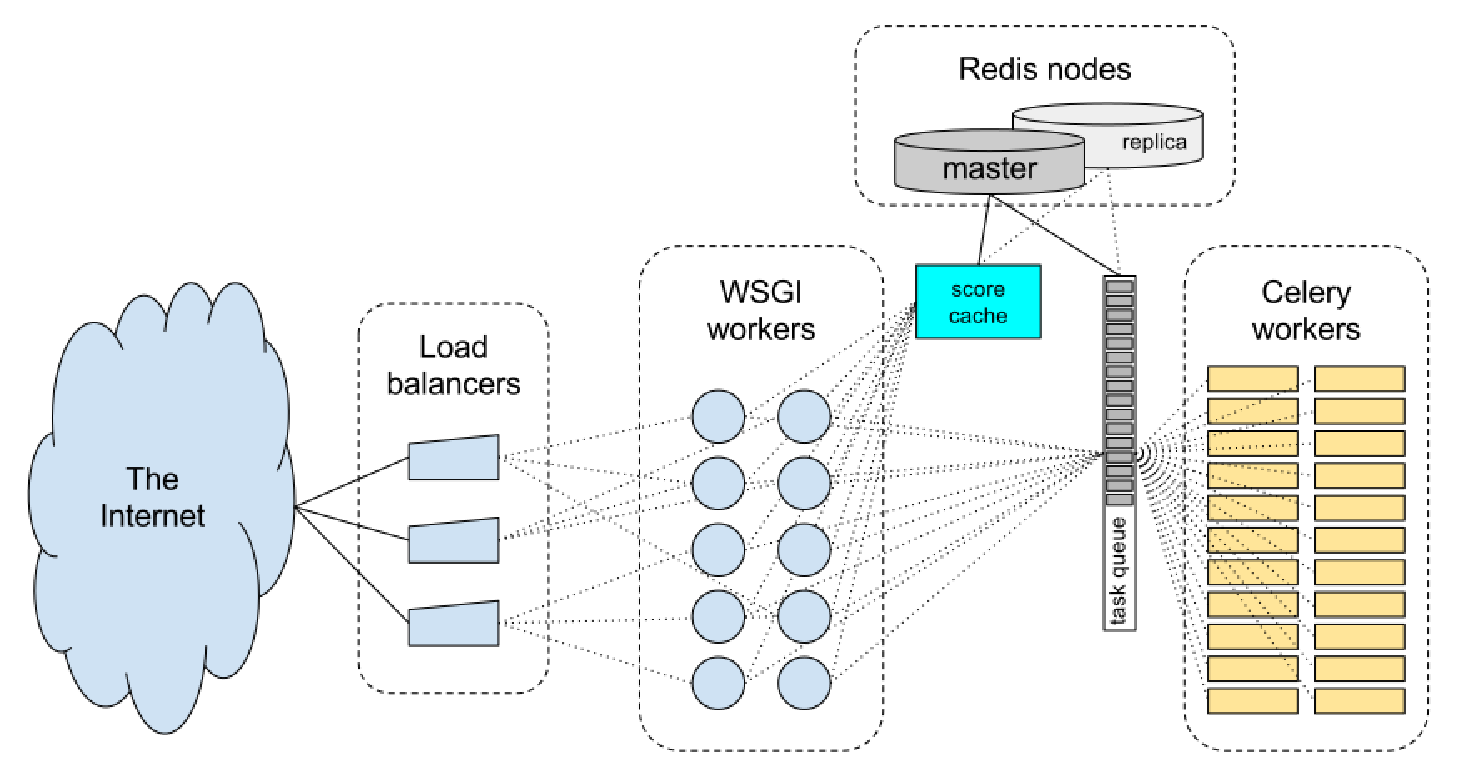
\includegraphics[width=.95\textwidth]{figures/ORES_architecture}
  \caption{ORES architectural overview}
  \label{fig:ores_architecture}
\end{figure}

ORES can be understood as a machine prediction model container service where the ``container'', referred to as a \emph{ScoringModel}, contains a set of dependency-aware features (see discussion of \emph{Dependency injection} in Section~\ref{sec:innovations_in_openness}) and has a common interface method called ``score()'' that takes the extracted feature-values as a parameter and produces a score as a JSON document.  The general ORES framework is responsible for extracting the features and serving the score object via a RESTful HTTP interface.  In this section we describe ORES architecture and how we have engineered the system to support our users' needs.

\subsection{Horizontal scaling}
In order to be a useful resource for Wikipedians and tool developers, the ORES system uses distributed computation strategies to serve a robust, fast, high-availability service.   In order to make sure that ORES can keep up with demand, we've focused on  two points at which the ORES system implements horizontal scale-ability: the input-output(IO) workers (uwsgi\footnote{\url{https://uwsgi-docs.readthedocs.io/}}) and the computation workers (celery\footnote{\url{http://www.celeryproject.org/}}).  When a request is received, it is split across the pool of available IO workers.  During this step of computation, all of the root dependencies are gathered for feature extraction using external APIs (e.g. the MediaWiki API\footnote{\url{http://enwp.org/:mw:MW:API}}).  Then these root dependencies are submitted to a job queue managed by \emph{celery} for the CPU-intensive work.  By implementing ORES in this way, we can add/remove new IO and CPU workers dynamically to the service in order to adjust with demand.

\subsection{Robustness}
Currently, IO workers and CPU workers are split across a set of 9 servers in two datacenters (for a total of 18 servers).  Each of these 9 servers are running 90 CPU workers and 135 IO workers.  The major limitation for running more workers on a single server is memory (RAM) due to the requirements for keeping several different prediction models loaded into memory.  IO and CPU workers are drawing from a shared queue, so other servers can take over should any individual go down.  Further, should one datacenter go fully offline, our load-balancer can detect this and will route traffic to the remaining datacenter.  This implements a high level of robustness and allows us to guarantee a high degree of uptime.  Given the relative youth of the ORES system and recent changes to the production configuration, it's difficult to give a fair estimate of the exact up-time percentage\footnote{\url{http://enwp.org/High_availability}}, but we've never experienced downtime that lasted more than a couple of hours.

\subsection{Batch processing}
Many of our users' use-cases involve the batch scoring of a large number of revisions.  E.g. when using ORES to build work-lists for Wikipedia editors, it's common to include an article quality prediction.  Work-lists are either built from the sum total of all 5m+ articles in Wikipedia or from some large subset specific to a single WikiProject (e.g. WikiProject Women Scientists claims about 6k articles\footnote{As demonstrated by \url{https://quarry.wmflabs.org/query/14033}}.).  Robots that maintain these worklists will periodically submit large batch processing jobs to score ORES once per day.  It's relevant to note that many researchers are also making use of ORES for varying historical analyses and their activity usually shows up in our logs as a sudden burst of requests.

The separation between IO and CPU work is very useful as it allows us to efficiently handle multi-score requests.  A request to score 50 revisions will be able to take advantage of batch IO during the first step of processing and still extract features for all 50 scores in parallel during the second CPU-intensive step.  This batch processing affords up to a 5X increase in time to scoring speed for large numbers of scores\cite{sarabadani2017building}.  We generally recommend that individuals looking to do batch processing with ORES submit requests in 50 score blocks using up to two parallel connections.  This would allow a user to easily score 1 million revisions in less than 24 hours in the worst case scenario that none of the scores were cached---which is unlikely for recent Wikipedia activity.

\subsection{Single score processing}
Many of our users' use-cases involve the request for a single score/prediction.  E.g. when using ORES for realtime counter-vandalism, tool developers will likely listen to a stream of edits as they are saved and submit a scoring request immediately.  It's critical that these requests return in a timely manner.  We implement several strategies to optimize this request pattern.

\leadin{Single score speed.}
In the worst case scenario, ORES is generating a score from scratch.  This is the common case when a score is requested in real-time---right after the target edit/article is saved.  We work to ensure that the median score duration is around 1 second.  Currently our metrics tracking suggests that for the week April 6-13th, our median, 75\%, and 95\% score response timings are 1.1, 1.2, and 1.9 seconds respectively.

\leadin{Caching and Precaching.}
In order to take advantage of the overlapping interests around recency between our users, we also maintain a basic LRU cache (using redis\footnote{\url{https://redis.io}}) using a deterministic score naming scheme (e.g. enwiki:123456:damaging would represent a score needed for the English Wikipedia damaging model for the edit identified by 123456).  This allows requests for scores that have recently been generated to be returned within about 50ms via HTTPS.

In order to make sure that scores for recent edits are available in the cache for real-time use-cases, we implement a ``precaching'' strategy that listens to a highspeed stream of recent activity in Wikipedia and automatically requests scores for a specific subset of actions (e.g. edits).  This allows us to attain a cache hit rate of about 80\% consistently.

There are also secondary caches of ORES scores implemented outside of our service.  E.g. the ORES Review Tool (an extension of MediaWiki) roughly mimics our own precaching strategy for gathering scores for recent edits in Wikipedia.  Since this cache and its access patterns are outside the metrics gathering system we use for the service, our cache hit rate is actually likely much higher than we're able to report.

\leadin{De-duplication}
In real-time use-cases of ORES, it is common that we will receive many requests to score the same edit/article right after it was saved.  We use the same deterministic score naming scheme from the cache to identify scoring tasks to ensure that simultaneous requests for that same score attach to the same result (or pending result) rather that starting a duplicate scoring job.  This pattern is very advantageous in the case of precaching, because of our network latency advantage: we can generally guarantee that the precaching request for a specific score precedes the external request for a score.  The result is that the external request for the a score attaches to the result of a score generation process that had started before the external request arrived.  So even worst case scenarios where the score is not yet generated often result in a better-than-expected response speed from the tool developer/users' point of view.

\subsection{Empirical access patterns}
\begin{figure*}[h]
\centering
\begin{subfigure}[t]{\textwidth}
  \centering
  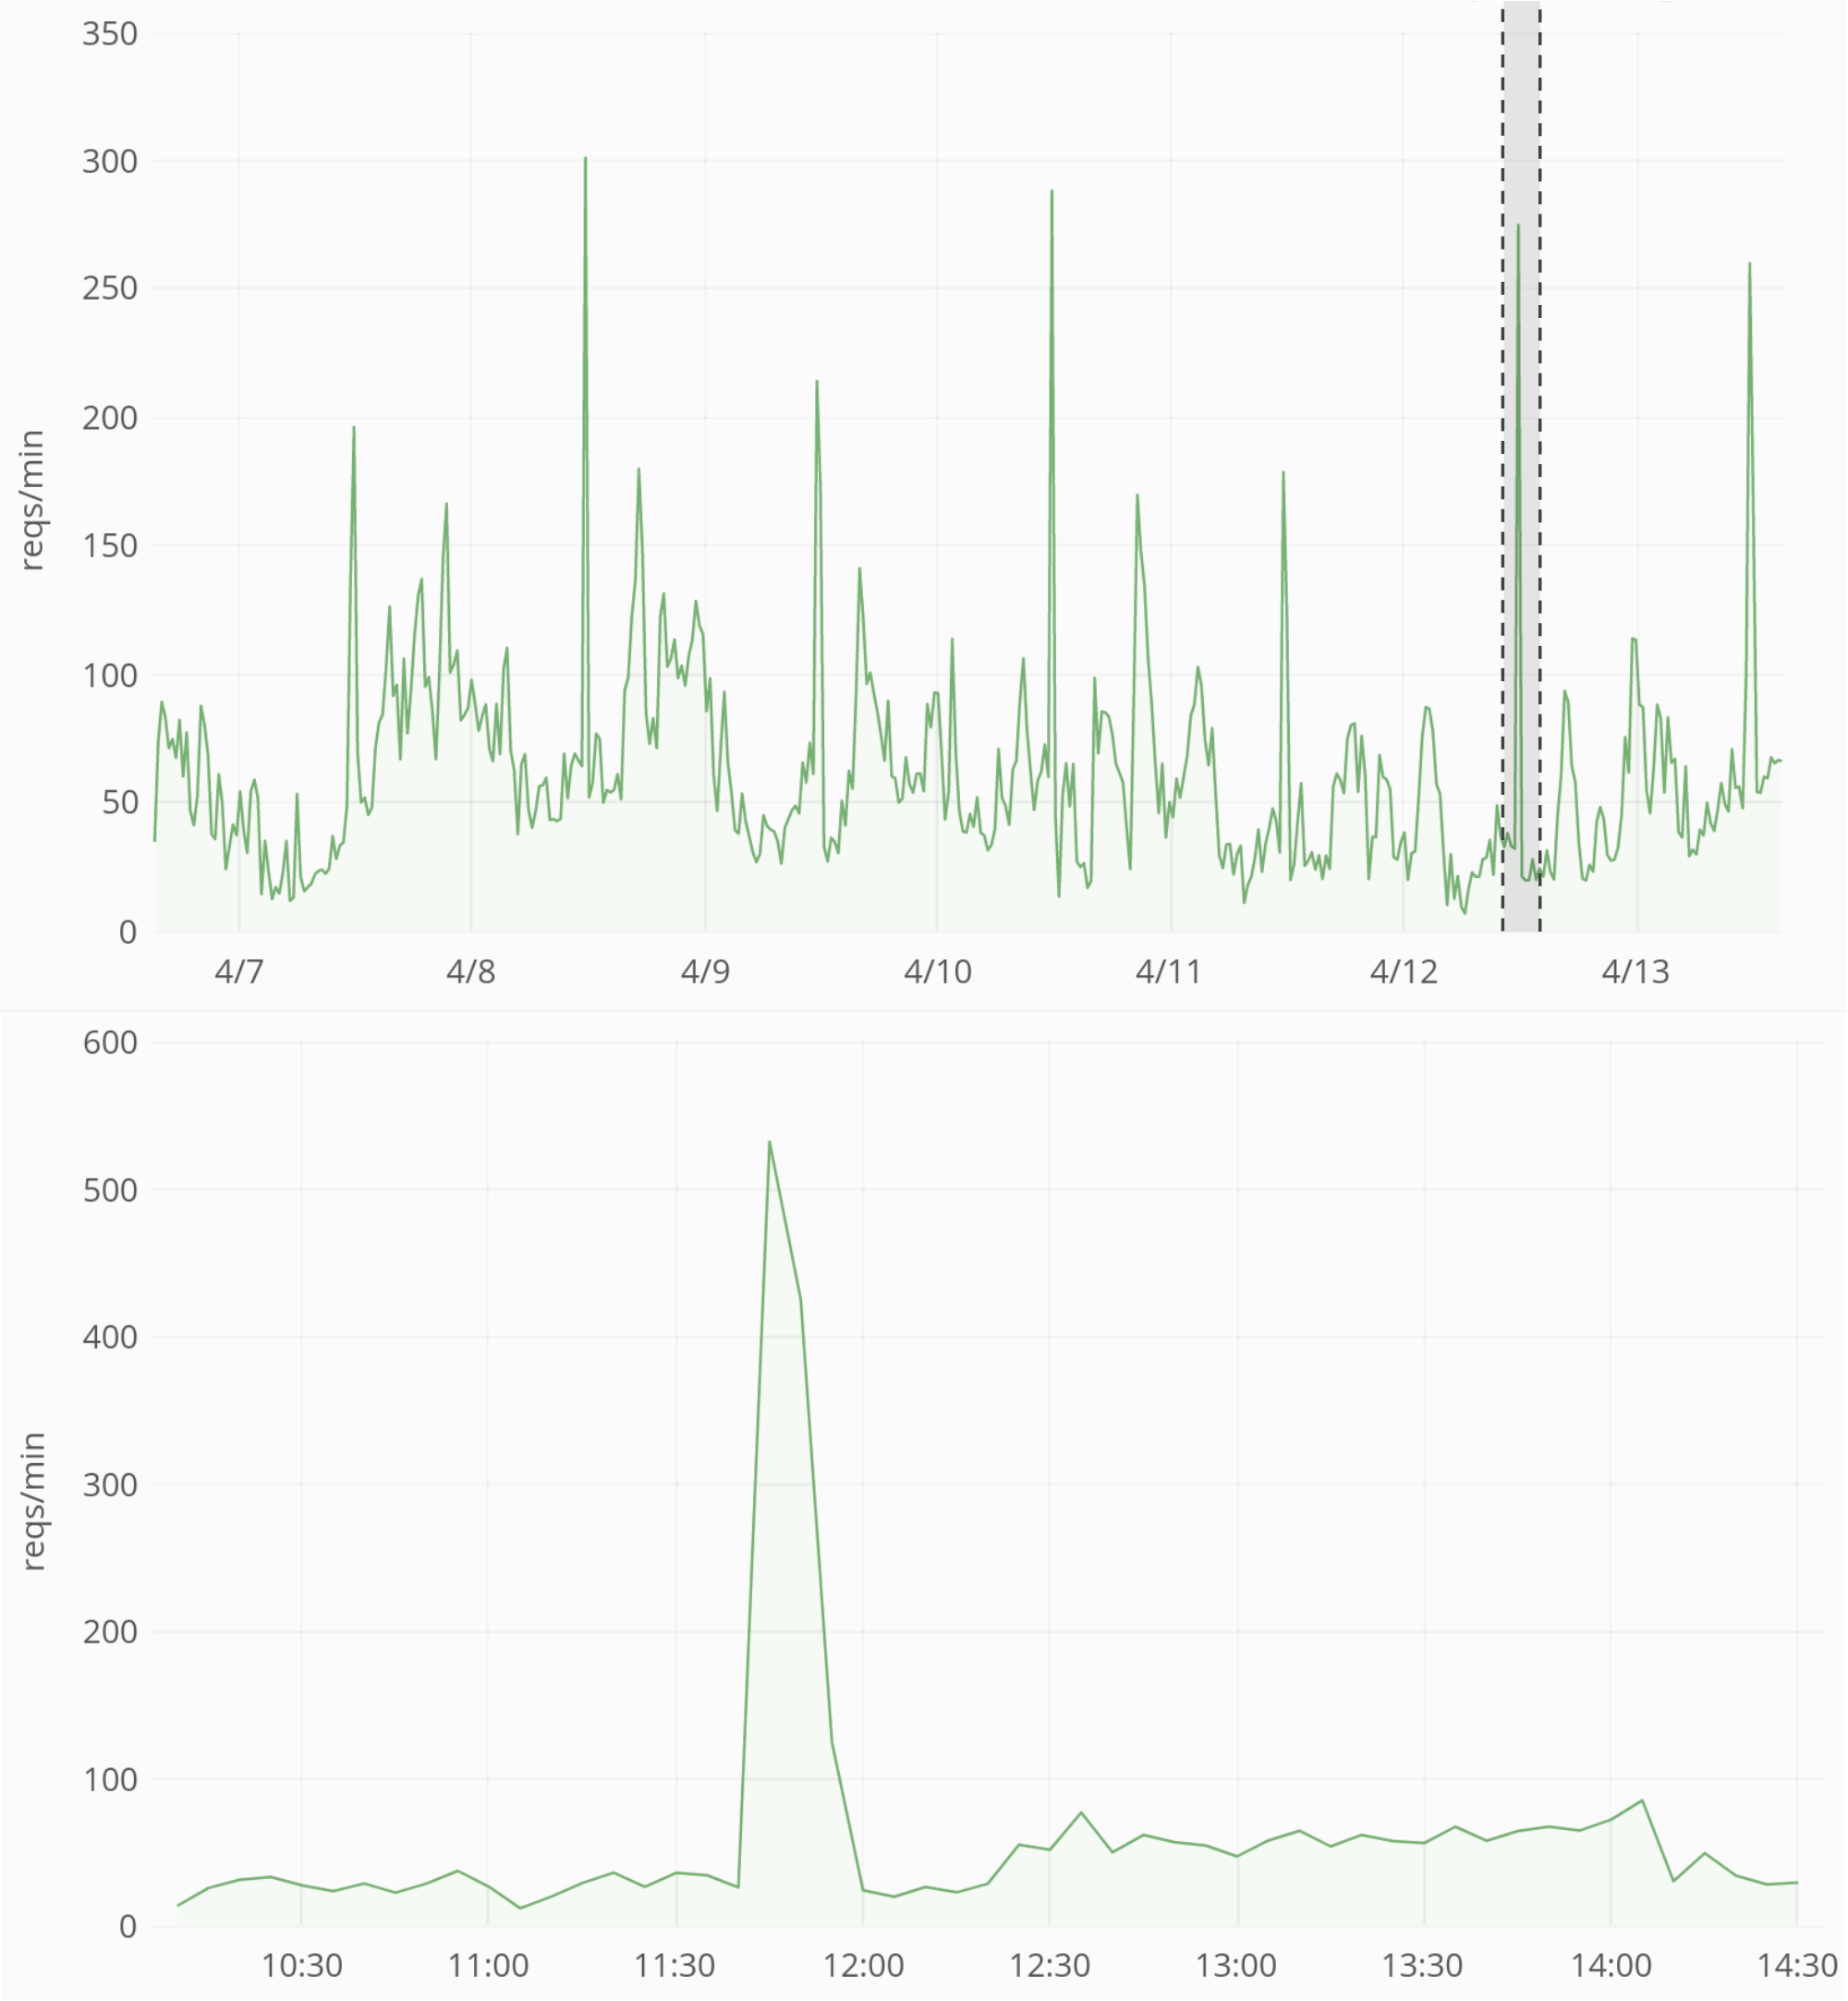
\includegraphics[width=.6\textwidth]{figures/ORES_request_activity_201804_week_vs_4hours}
  \caption{External requests per minute with a 4 hour block broken out to highlight a sudden burst of requests.}
  \label{fig:ores_request_rate}
\end{subfigure}\\
\begin{subfigure}[t]{\columnwidth}
  \centering
  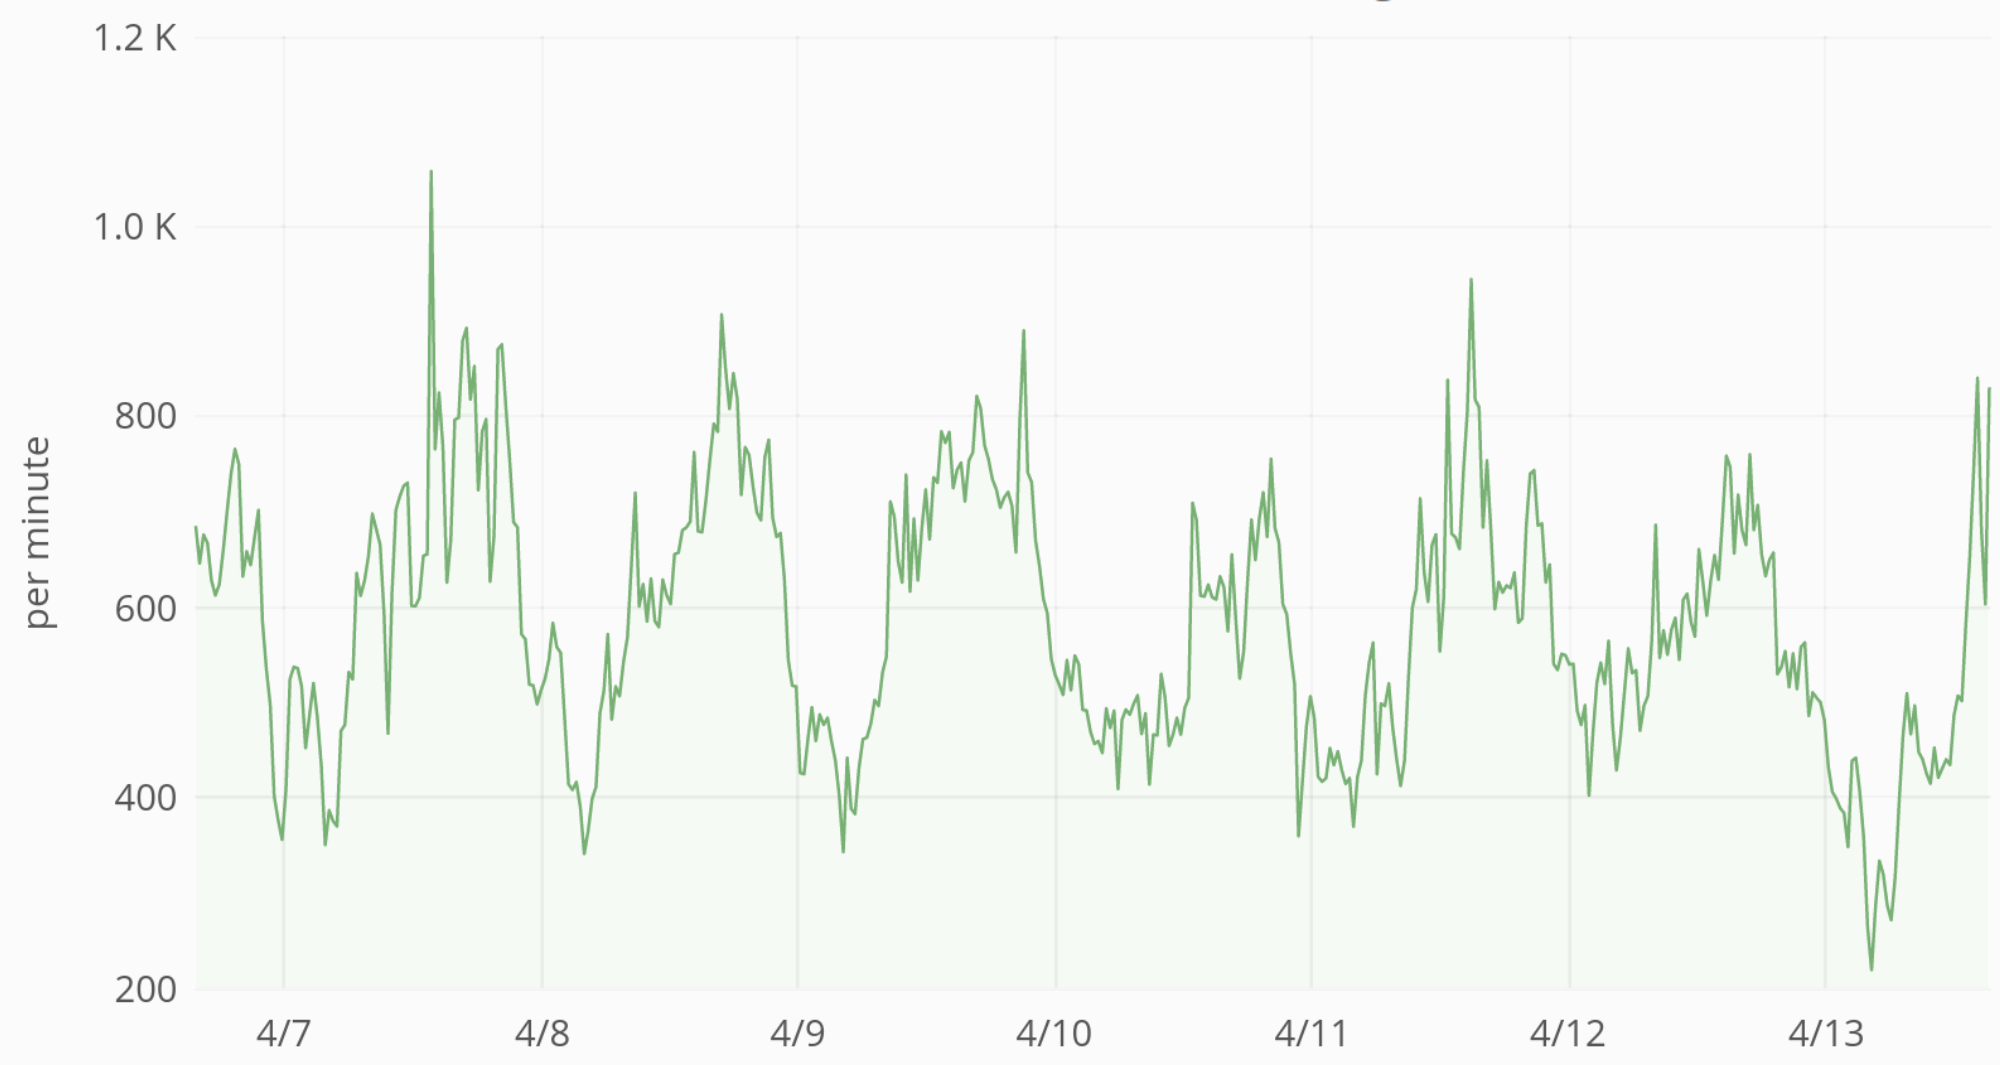
\includegraphics[width=.6\textwidth]{figures/ORES_precache_request_rate_201804}
  \caption{Precaching requests per minute}
  \label{fig:ores_precache_rate}
\end{subfigure}
\caption{Request rates to the ORES service for the week ending on April 13th, 2018}
\label{fig:ores_activity}
\end{figure*}


The ORES service has been online since July of 2015\cite{halfaker2015artificial}.  Since then, we have seen steadily rising usage as we've developed and deployed new models.  Currently, ORES support 66 different models for 33 different language-specific wikis.

Generally, we see 50 to 125 requests per minute from external tools that are using ORES' predictions (excluding the MediaWiki extension that is more difficult to track).  Sometimes these external requests will burst up to 400-500 requests per second.  Figure~\ref{fig:ores_request_rate} shows the periodic and bursty nature of scoring requests received by the ORES service.  Note that every day at about 11:40 UTC, the request rate jumps as some batch scoring job---most likely a bot.

Figure~\ref{fig:ores_precache_rate} shows our rate of precaching requests coming from our own systems.  This graph roughly reflects the rate of edits that are happening to all of the wikis that we support since we'll start a scoring job for nearly every edit as it happens.  Note that the number of precaching requests is about an order of magnitude higher than our known external score request rate.  This is expected since Wikipedia editors and the tools they use will not request a score for every single revisions.  It is the computational price that we pay to attain a high cache hit rate and to ensure that our users get the quickest response possible for the scores that they \emph{do} need.
